% Protocolo PERS sobre RWS (un tramo) -- compilar con: pdflatex fig_secuencia.tex
\documentclass[border=1pt]{standalone}
\usepackage[T1]{fontenc}
\usepackage[utf8]{inputenc}
\usepackage{mathptmx}
\renewcommand{\ttdefault}{lmtt}
\usepackage{tikz}
\usetikzlibrary{arrows.meta,calc}
\begin{document}
\scriptsize
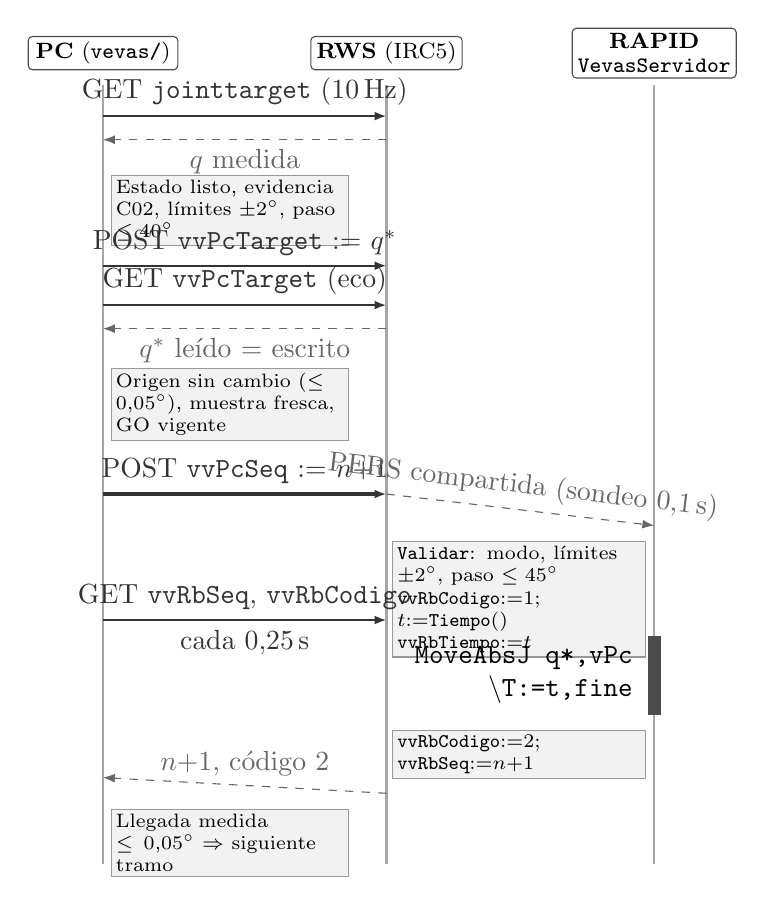
\begin{tikzpicture}[
  y=-1mm,
  msg/.style={-{Latex[length=1.5mm]}, thick, black!80},
  rsp/.style={-{Latex[length=1.5mm]}, dashed, black!60},
  nota/.style={draw=black!40, fill=black!5, align=left, inner sep=1.6pt, font=\scriptsize},
  cab/.style={draw=black!70, fill=white, rounded corners=1.5pt, align=center, inner sep=2pt, font=\footnotesize, minimum width=19mm}]
\def\xa{0} \def\xb{36} \def\xc{70}
\node[cab] (A) at (\xa mm, 0) {\textbf{PC} (\texttt{vevas/})};
\node[cab] (B) at (\xb mm, 0) {\textbf{RWS} (IRC5)};
\node[cab] (C) at (\xc mm, 0) {\textbf{RAPID}\\[-1pt]\texttt{VevasServidor}};
\foreach \x in {\xa,\xb,\xc} \draw[black!35, thick] (\x mm, 4) -- (\x mm, 103);

% 1 lectura periódica
\draw[msg] (\xa mm, 8) -- node[above, pos=0.5] {GET \texttt{jointtarget} (10\,Hz)} (\xb mm, 8);
\draw[rsp] (\xb mm, 11) -- node[below] {$q$ medida} (\xa mm, 11);
% 2 chequeos PC
\node[nota, anchor=north west, text width=29mm] at (\xa mm + 1mm, 15.5) {Estado listo, evidencia C02, límites $\pm2^\circ$, paso $\le 40^\circ$};
% 3 objetivo y lectura de vuelta
\draw[msg] (\xa mm, 27) -- node[above] {POST \texttt{vvPcTarget} := $q^\ast$} (\xb mm, 27);
\draw[msg] (\xa mm, 32) -- node[above] {GET \texttt{vvPcTarget} (eco)} (\xb mm, 32);
\draw[rsp] (\xb mm, 35) -- node[below] {$q^\ast$ leído $=$ escrito} (\xa mm, 35);
\node[nota, anchor=north west, text width=29mm] at (\xa mm + 1mm, 40) {Origen sin cambio ($\le 0{,}05^\circ$), muestra fresca, GO vigente};
% 4 orden
\draw[msg, very thick] (\xa mm, 56) -- node[above] {POST \texttt{vvPcSeq} := $n{+}1$} (\xb mm, 56);
\draw[rsp] (\xb mm, 56) -- node[above, align=center, sloped] {PERS compartida (sondeo 0,1\,s)} (\xc mm, 60);
% 5 RAPID
\node[nota, anchor=north east, text width=31mm] at (\xc mm - 1mm, 62) {\texttt{Validar}: modo, límites $\pm2^\circ$, paso $\le45^\circ$\\
\texttt{vvRbCodigo}:=1;\; $t$:=\texttt{Tiempo}()\\ \texttt{vvRbTiempo}:=$t$};
\fill[black!70] (\xc mm - 0.8mm, 74) rectangle (\xc mm + 0.8mm, 84);
\node[anchor=east, align=right] at (\xc mm - 1.5mm, 79) {\texttt{MoveAbsJ q*,vPc}\\\texttt{\textbackslash T:=t,fine}};
\node[nota, anchor=north east, text width=31mm] at (\xc mm - 1mm, 86) {\texttt{vvRbCodigo}:=2;\; \texttt{vvRbSeq}:=$n{+}1$};
% 6 sondeo del PC
\draw[msg] (\xa mm, 72) -- node[above] {GET \texttt{vvRbSeq}, \texttt{vvRbCodigo}} node[below] {cada 0,25\,s} (\xb mm, 72);
\draw[rsp] (\xb mm, 94) -- node[above] {$n{+}1$, código 2} (\xa mm, 92);
\node[nota, anchor=north west, text width=29mm] at (\xa mm + 1mm, 96) {Llegada medida $\le 0{,}05^\circ$ $\Rightarrow$ siguiente tramo};
\end{tikzpicture}
\end{document}
